\section*{Research problems}
\addcontentsline{toc}{section}{\protect\numberline{}{Research problems}}

% Our scope
Formally, we consider the optimal \emph{sequence-to-graph alignment} problem,
the task of finding an optimal base-to-base correspondence between a query
sequence and a (possibly cyclic) walk in the graph. Related alignment problems
have already been formulated as graph shortest path
problems~\cite{jain_complexity_2019}.

\paragraph{Alignment problem}
% problem statements
We consider the problem of pairwise sequence alignment in the context of genomic
data: given two DNA sequences, one has to be aligned to the other. It would have
been a rather trivial task if the alignment would be perfect. Nevertheless, the
real data contains both biological variation and technical errors resulting from
evolution and the sequencing process. A common intuitive and robust assumption
is that an alignment with a minimal number of single-letter edits
(substitutions, insertions and deletions) is the most plausable explainationo of
the divergence of both sequences from an unknown common ancestor.

% alignment types
\begin{figure}[t]  %\begin{floatingfigure}[l]{0.5\textwidth}
    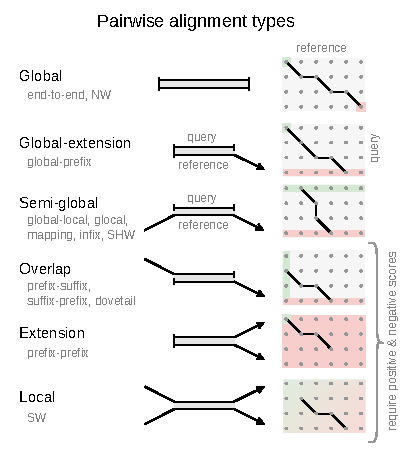
\includegraphics[width=0.5\textwidth]{alignment-types}
	\caption[Alignment types]{Alignment types.}
    \label{fig:alignment-types}
\end{figure}
\paragraph{Global and semi-global alignment}
Two sequences can be aligned in multiple ways (\cref{fig:alignment-types}). In
this thesis we focus on global and semi-global alignment types only. If both
sequences have to be aligned end to end, we look for a \emph{global alignment}
whose minimal number of edits is known as \emph{edit distance}. If we instead
search for an occurance of a query sequence within a reference sequence, we
allow the alignment to start and end at any reference locations in a
\emph{semi-global} alignment (also called approximate/fuzzy string search
outside computational biology).

%\paragraph{Problem statement}
%\paragraph{Problem domain}

\paragraph{Semi-global alignment}

% General: aligning, edit distance
Alignment of reads to a reference genome is an essential and early step in most
bioinformatics pipelines. While linear references have been used traditionally,
an increasing interest is directed towards graph references capable of
representing biological variation~\citep{garrison_variation_2018}.
%
Specifically, a \emph{sequence-to-graph} alignment is a base-to-base
correspondence between a given read and a walk in the graph. As sequencing
errors and biological variation result in inexact read alignments, edit distance
is the most common metric that alignment algorithms optimize in order to find
the most probable read origin in the reference.

% We note that in contrast to linear references, reference graphs capture
% genomic variation and therefore enable more accurate
% alignments~\citep{garrison_variation_2018}.

% paper-trie; seed-and-extend approach to semi-global alignment

\paragraph{Pangenomes and reference graphs}

The shortest path approach naturally fits more complex references than linear.
In fact, any graph reference (incl. cycles) is fine.

% paper-trie; Accounting for variation
%\paragraph{Accounting for Variation}
First attempts to include variation into the reference data structure were made
by augmenting the local alignment method to consider alternative walks during the
extend step~\cite{schneeberger_simultaneous_2009,palmapper}. This approach has
since been extended from the linear reference case to graph references. To
represent non-reference variation of multiple references during the seeding
stage, HISAT2 uses generalized compressed suffix
arrays~\cite{siren_indexing_2014} to index walks in an augmented reference
sequence, forming a local genome graph~\cite{kim_graphbased_2019}.
VG~\cite{garrison_variation_2018} uses a similar
technique~\cite{siren_indexing_2017} to index variation graphs representing a
population of references.

% paper-trie; The benefit from genome graphs
Historically, a single linear reference sequence has been used to represent the
most common variants in a population. While providing a working abstraction for
most cases, rare or sub-population specific variation is especially hard to
model in this setting, creating a reference allele
bias~\cite{stevenson_sources_2013,brandt_mapping_2015}. Consequently, in the
last few years, the field has shifted first towards using sets of reference
sequences, and more recently to graph data structures (so-called {\em genome
graphs}), to represent many genomes or haplotypes
simultaneously~\cite{dilthey_improved_2015,paten_genome_2017,garrison_variation_2018}.

% Sequencing and variant calling
The analysis and understanding of genetic variation encoded in the genome of an
organism lies at the center of computational biology and medicine. Variation is
usually identified through matching sequences obtained from DNA/RNA-sequencing
back to a reference (genome) sequence in the process of \emph{variant calling},
making the alignment task a core problem in sequence bioinformatics.

\subsection*{Global alignment}
% paper:seeds
%\subsection{Problem statement: Alignment as shortest path} \label{SEEDsec:task}
%

%\section{Task Description: Alignment to Reference Graphs}
\label{TRIEsec:task}

\paragraph{Scalable optimal alignment}
